% Created 2021-05-31 Mon 23:37
% Intended LaTeX compiler: pdflatex
\documentclass[11pt]{article}
\usepackage[utf8]{inputenc}
\usepackage[T1]{fontenc}
\usepackage{graphicx}
\usepackage{grffile}
\usepackage{longtable}
\usepackage{wrapfig}
\usepackage{rotating}
\usepackage[normalem]{ulem}
\usepackage{amsmath}
\usepackage{textcomp}
\usepackage{amssymb}
\usepackage{capt-of}
\usepackage{hyperref}
\usepackage[top=1in, bottom=1.25in, left=1.25in, right=1.25in]{geometry}
\usepackage{parskip}
\usepackage[style=ieee,hyperref=true,backref=true,url=true,backend=biber,natbib=true]{biblatex}
\addbibresource{ref.bib}
\usepackage{chessboard}
\ExplSyntaxOn %requires texlive 2020, in older system load expl3
\cs_new:Npn \getfieldnumber #1
{
\fp_eval:n { (\tl_tail:V #1 -1)*8 + \exp_args:Ne\int_from_alph:n{\tl_head:V #1} -1}
}
\ExplSyntaxOff

\usepackage[main,include]{embedall}
\IfFileExists{./\jobname.org}{\embedfile[desc=The original file]{\jobname.org}}{}





\usepackage{fvextra}
\fvset{
  commandchars=\\\{\},
  highlightcolor=white!95!black!80!blue,
  breaklines=true,
  breaksymbol=\color{white!60!black}\tiny\ensuremath{\hookrightarrow},
}
\renewcommand\theFancyVerbLine{\footnotesize\color{black!40!white}\arabic{FancyVerbLine}}

\usepackage[many]{tcolorbox}
\DeclareTColorBox[]{Code}{}%
{enhanced,
  colback=white!97!black,
  colframe=white!94!black, boxrule=0.5pt,
  fontupper=\color{EFD}\footnotesize,
  arc=2.5pt, outer arc=2.5pt,
  boxsep=2pt, left=2pt, right=2pt, top=1pt, bottom=0.5pt,
  breakable}

\definecolor{EFD}{HTML}{383a42}
\newcommand{\EFD}[1]{\textcolor{EFD}{#1}} % default
\definecolor{EFk}{HTML}{e45649}
\newcommand{\EFk}[1]{\textcolor{EFk}{#1}} % font-lock-keyword-face
\definecolor{EFd}{HTML}{84888b}
\newcommand{\EFd}[1]{\textcolor{EFd}{\textit{#1}}} % font-lock-doc-face
\definecolor{EFt}{HTML}{986801}
\newcommand{\EFt}[1]{\textcolor{EFt}{#1}} % font-lock-type-face
\definecolor{EFs}{HTML}{50a14f}
\newcommand{\EFs}[1]{\textcolor{EFs}{#1}} % font-lock-string-face
\definecolor{EFw}{HTML}{986801}
\newcommand{\EFw}[1]{\textcolor{EFw}{#1}} % font-lock-warning-face
\definecolor{EFb}{HTML}{a626a4}
\newcommand{\EFb}[1]{\textcolor{EFb}{#1}} % font-lock-builtin-face
\definecolor{EFct}{HTML}{9ca0a4}
\newcommand{\EFct}[1]{\textcolor{EFct}{#1}} % font-lock-comment-face
\definecolor{EFc}{HTML}{b751b6}
\newcommand{\EFc}[1]{\textcolor{EFc}{#1}} % font-lock-constant-face
\definecolor{EFpp}{HTML}{4078f2}
\newcommand{\EFpp}[1]{\textcolor{EFpp}{\textbf{#1}}} % font-lock-preprocessor-face
\definecolor{EFnc}{HTML}{4078f2}
\newcommand{\EFnc}[1]{\textcolor{EFnc}{\textbf{#1}}} % font-lock-negation-char-face
\definecolor{EFv}{HTML}{6a1868}
\newcommand{\EFv}[1]{\textcolor{EFv}{#1}} % font-lock-variable-name-face
\definecolor{EFf}{HTML}{a626a4}
\newcommand{\EFf}[1]{\textcolor{EFf}{#1}} % font-lock-function-name-face
\definecolor{EFcd}{HTML}{9ca0a4}
\newcommand{\EFcd}[1]{\textcolor{EFcd}{#1}} % font-lock-comment-delimiter-face
\definecolor{EFrc}{HTML}{4078f2}
\newcommand{\EFrc}[1]{\textcolor{EFrc}{\textbf{#1}}} % font-lock-regexp-grouping-construct
\definecolor{EFrb}{HTML}{4078f2}
\newcommand{\EFrb}[1]{\textcolor{EFrb}{\textbf{#1}}} % font-lock-regexp-grouping-backslash
\definecolor{EFhn}{HTML}{da8548}
\newcommand{\EFhn}[1]{\textcolor{EFhn}{\textbf{#1}}} % highlight-numbers-number
\definecolor{EFhq}{HTML}{4078f2}
\newcommand{\EFhq}[1]{\textcolor{EFhq}{#1}} % highlight-quoted-quote
\definecolor{EFhs}{HTML}{986801}
\newcommand{\EFhs}[1]{\textcolor{EFhs}{#1}} % highlight-quoted-symbol
\definecolor{EFrdi}{HTML}{4078f2}
\newcommand{\EFrdi}[1]{\textcolor{EFrdi}{#1}} % rainbow-delimiters-depth-1-face
\definecolor{EFrdii}{HTML}{a626a4}
\newcommand{\EFrdii}[1]{\textcolor{EFrdii}{#1}} % rainbow-delimiters-depth-2-face
\definecolor{EFrdiii}{HTML}{50a14f}
\newcommand{\EFrdiii}[1]{\textcolor{EFrdiii}{#1}} % rainbow-delimiters-depth-3-face
\definecolor{EFrdiv}{HTML}{da8548}
\newcommand{\EFrdiv}[1]{\textcolor{EFrdiv}{#1}} % rainbow-delimiters-depth-4-face
\definecolor{EFrdv}{HTML}{b751b6}
\newcommand{\EFrdv}[1]{\textcolor{EFrdv}{#1}} % rainbow-delimiters-depth-5-face
\definecolor{EFrdvi}{HTML}{986801}
\newcommand{\EFrdvi}[1]{\textcolor{EFrdvi}{#1}} % rainbow-delimiters-depth-6-face
\definecolor{EFrdvii}{HTML}{4db5bd}
\newcommand{\EFrdvii}[1]{\textcolor{EFrdvii}{#1}} % rainbow-delimiters-depth-7-face
\definecolor{EFrdiix}{HTML}{80a880}
\newcommand{\EFrdiix}[1]{\textcolor{EFrdiix}{#1}} % rainbow-delimiters-depth-8-face
\definecolor{EFrdix}{HTML}{887070}
\newcommand{\EFrdix}[1]{\textcolor{EFrdix}{#1}} % rainbow-delimiters-depth-9-face
\author{Jake Moss - s46409665}
\date{\today}
\title{Chess game animation in blender}
\hypersetup{
 pdfauthor={Jake Moss - s46409665},
 pdftitle={Chess game animation in blender},
 pdfkeywords={},
 pdfsubject={},
 pdfcreator={Emacs 28.0.50 (Org mode 9.5)}, 
 pdflang={English}}
\begin{document}

\maketitle
\tableofcontents

\newpage

\section{Introduction}
\label{sec:orgf6461a5}
\subsection{Project aims}
\label{sec:org4c663ca}
\section{The idea}
\label{sec:org375cbe3}
\section{Implementation}
\label{sec:org5b1f7f0}
\subsection{Blender side}
\label{sec:org77210c7}
\subsubsection{Piece modelling}
\label{sec:org3ab0387}
Pieces were modelled after the reference image below Figure \ref{piece-reference}. From this image the pieces where traced using the \texttt{Add Vertex} tool, from the \href{https://docs.blender.org/manual/en/2.92/addons/add\_mesh/mesh\_extra\_objects.html}{Add Mess Extra Objects} add-on. To transform this line of vertices to a solid object  a \texttt{Screw} modifier was applied.
\begin{figure}[htbp]
\centering
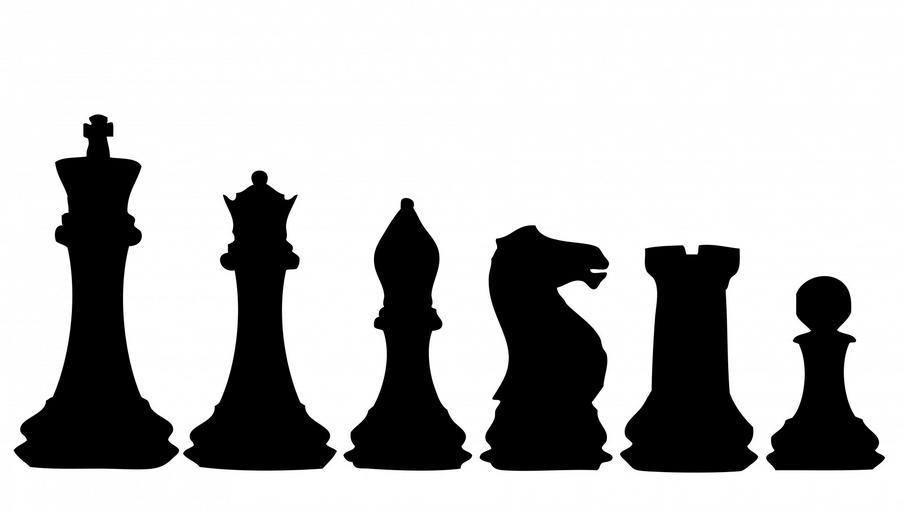
\includegraphics[width=0.5\textwidth]{ref/bee5aa3d08a30da4ca1005cbd0fe10b54a03bb49.jpg}
\caption{\label{piece-reference}Reference image, Licensed under \href{https://pixabay.com/service/license/}{Pixabay License}}
\end{figure}

\begin{center}
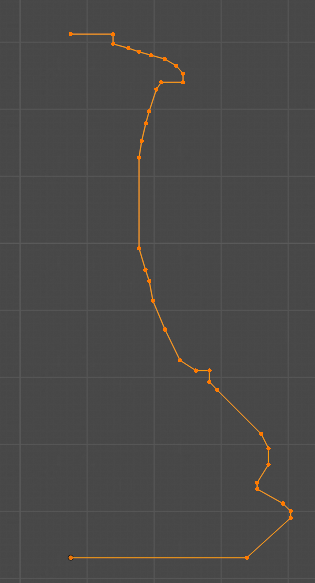
\includegraphics[height=150pt]{Images/modelling piece inprogress.png}
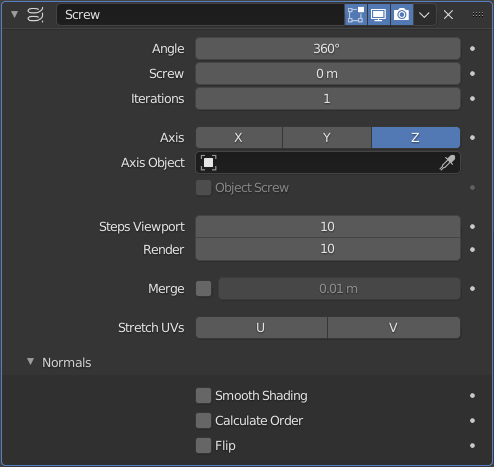
\includegraphics[height=150pt]{Images/screw settings.png}
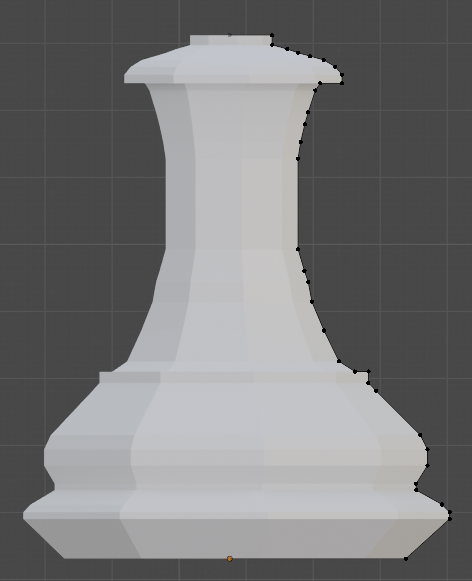
\includegraphics[height=150pt]{Images/pawn model.png}
\end{center}
The notable changes from the default settings is the lowering of the steps from
\(16 \to 10\) and disabling \texttt{Smooth Shading}. This was a stylistic choice as it
was believed that the low polygon look would better demonstration reflections and
the planned indirect lighting (see \hyperref[sec:org0755980]{Lighting - Disco Ball}).

To model the knight, 3 seperate reference images where used.
\begin{center}
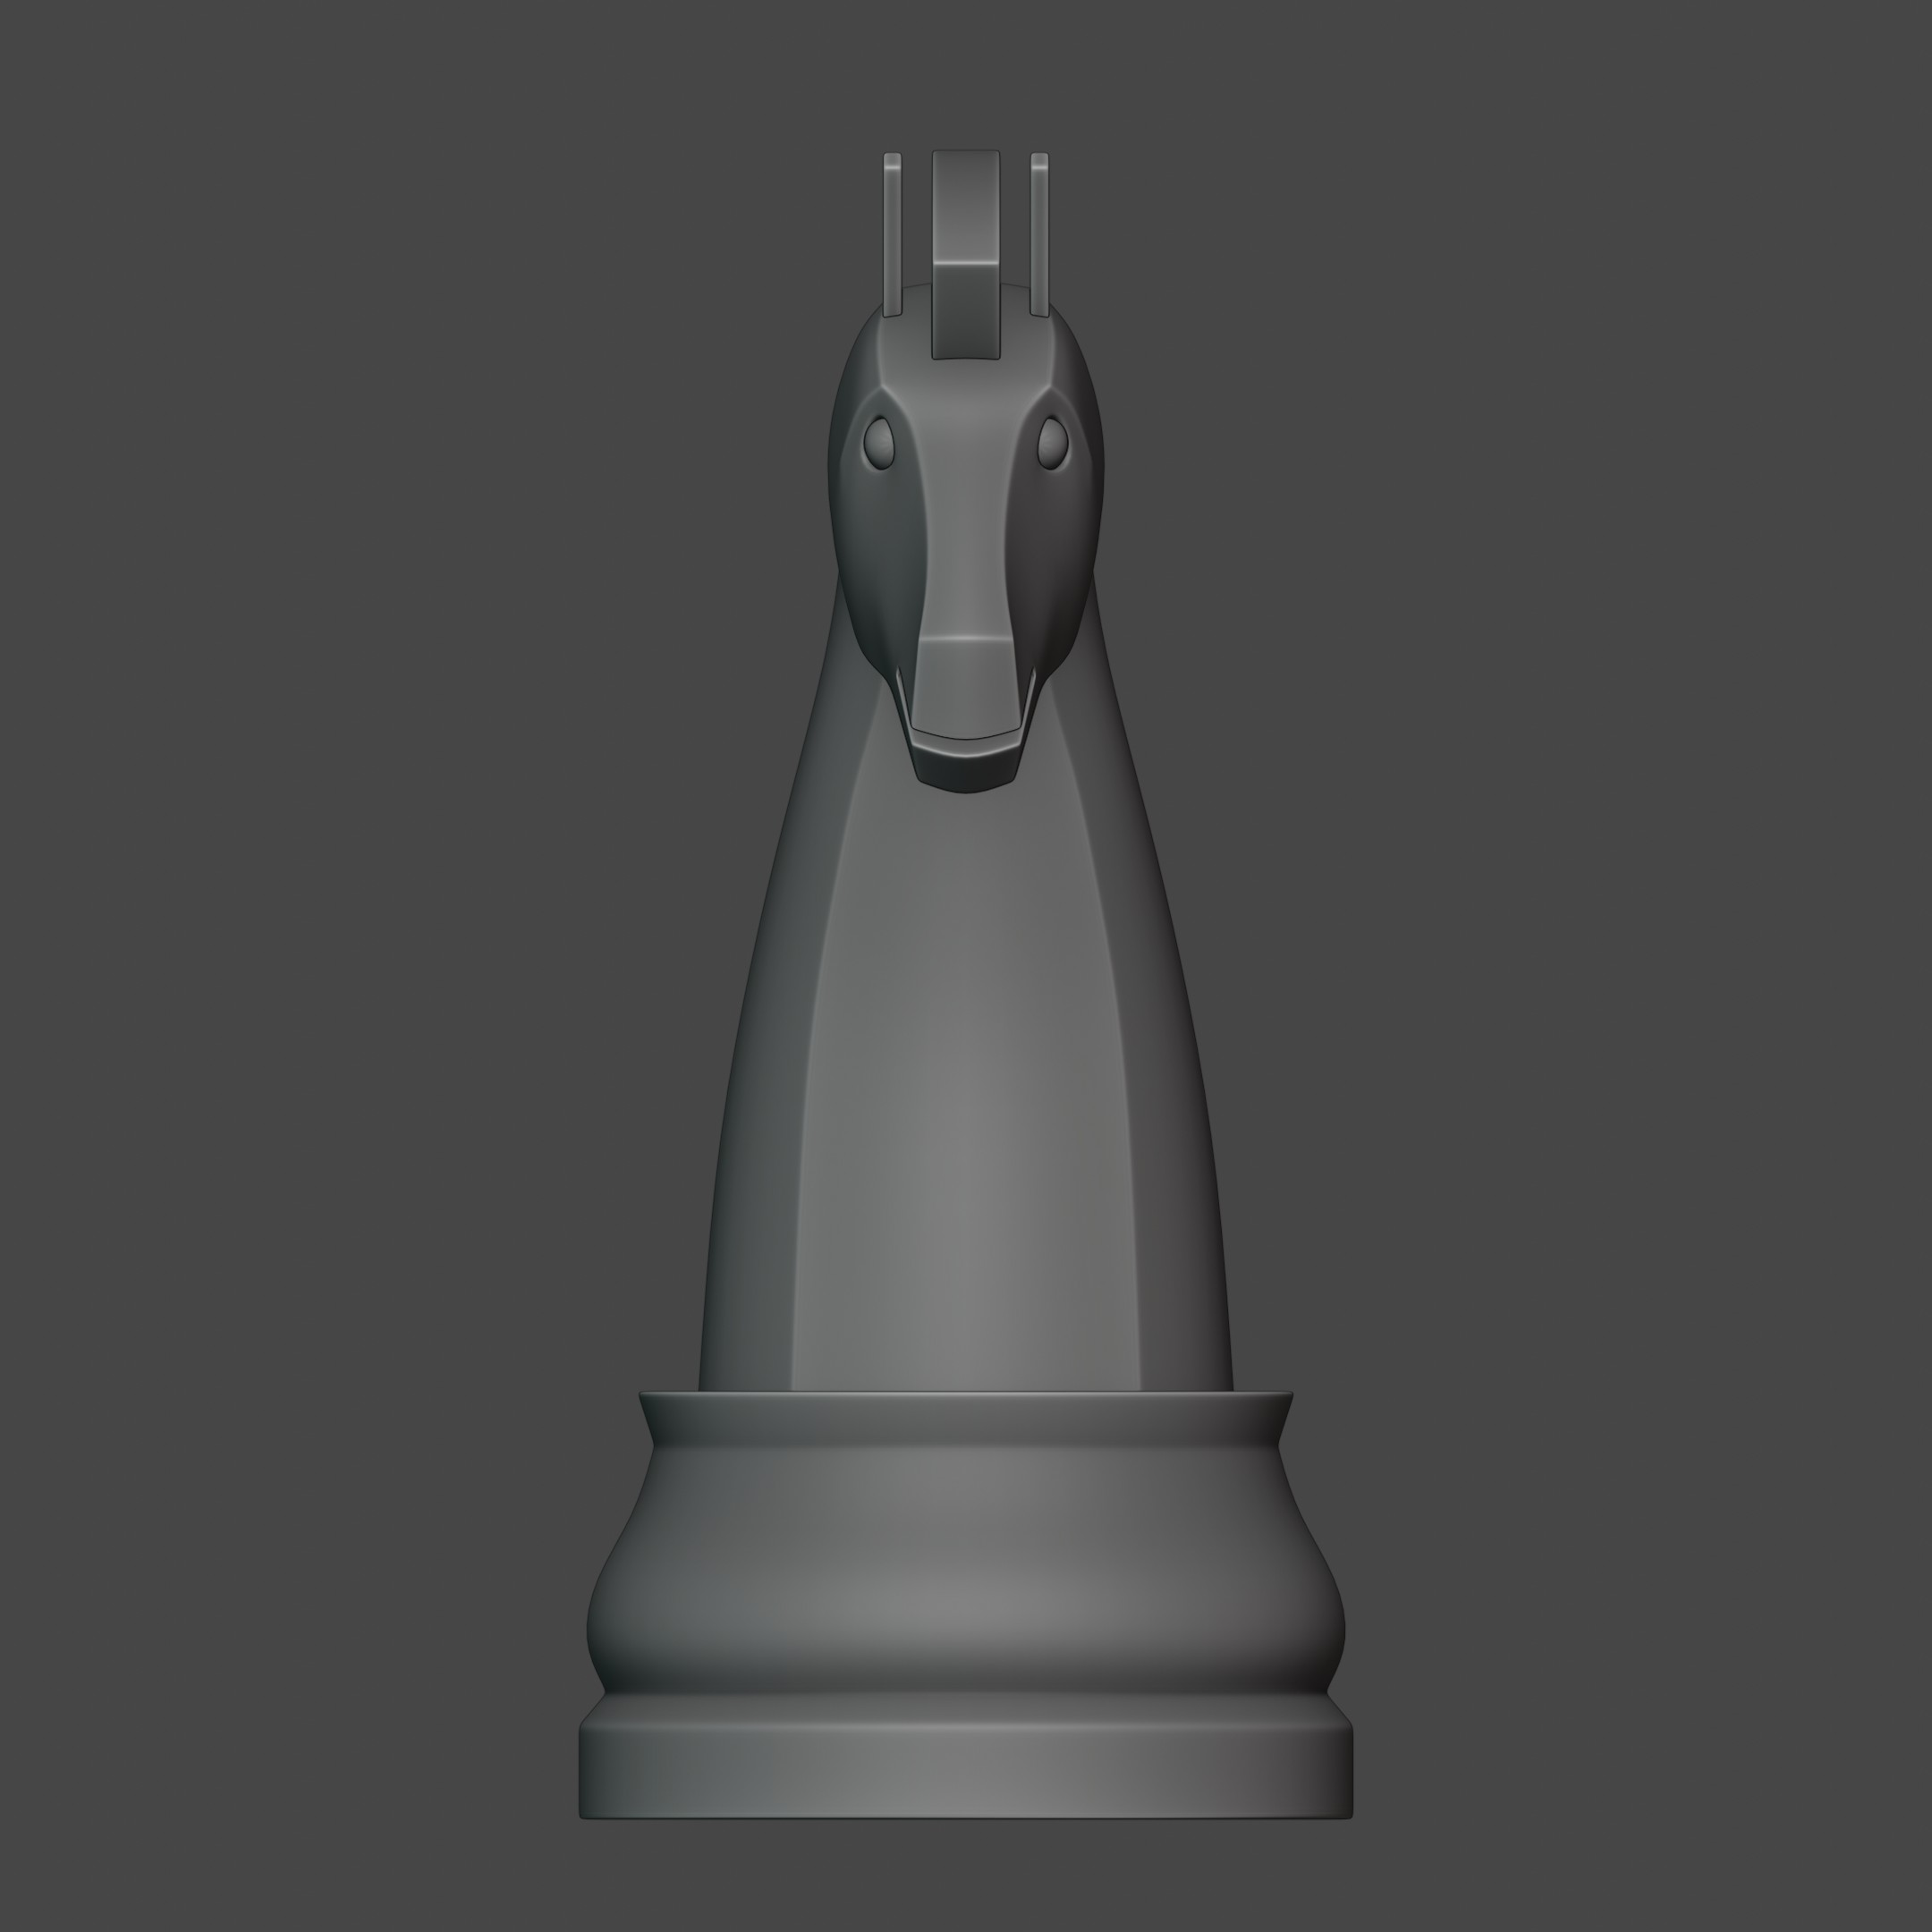
\includegraphics[width=0.3\textwidth]{ref/knight front.jpg}

\includegraphics[width=0.3\textwidth]{ref/knight right.jpg}
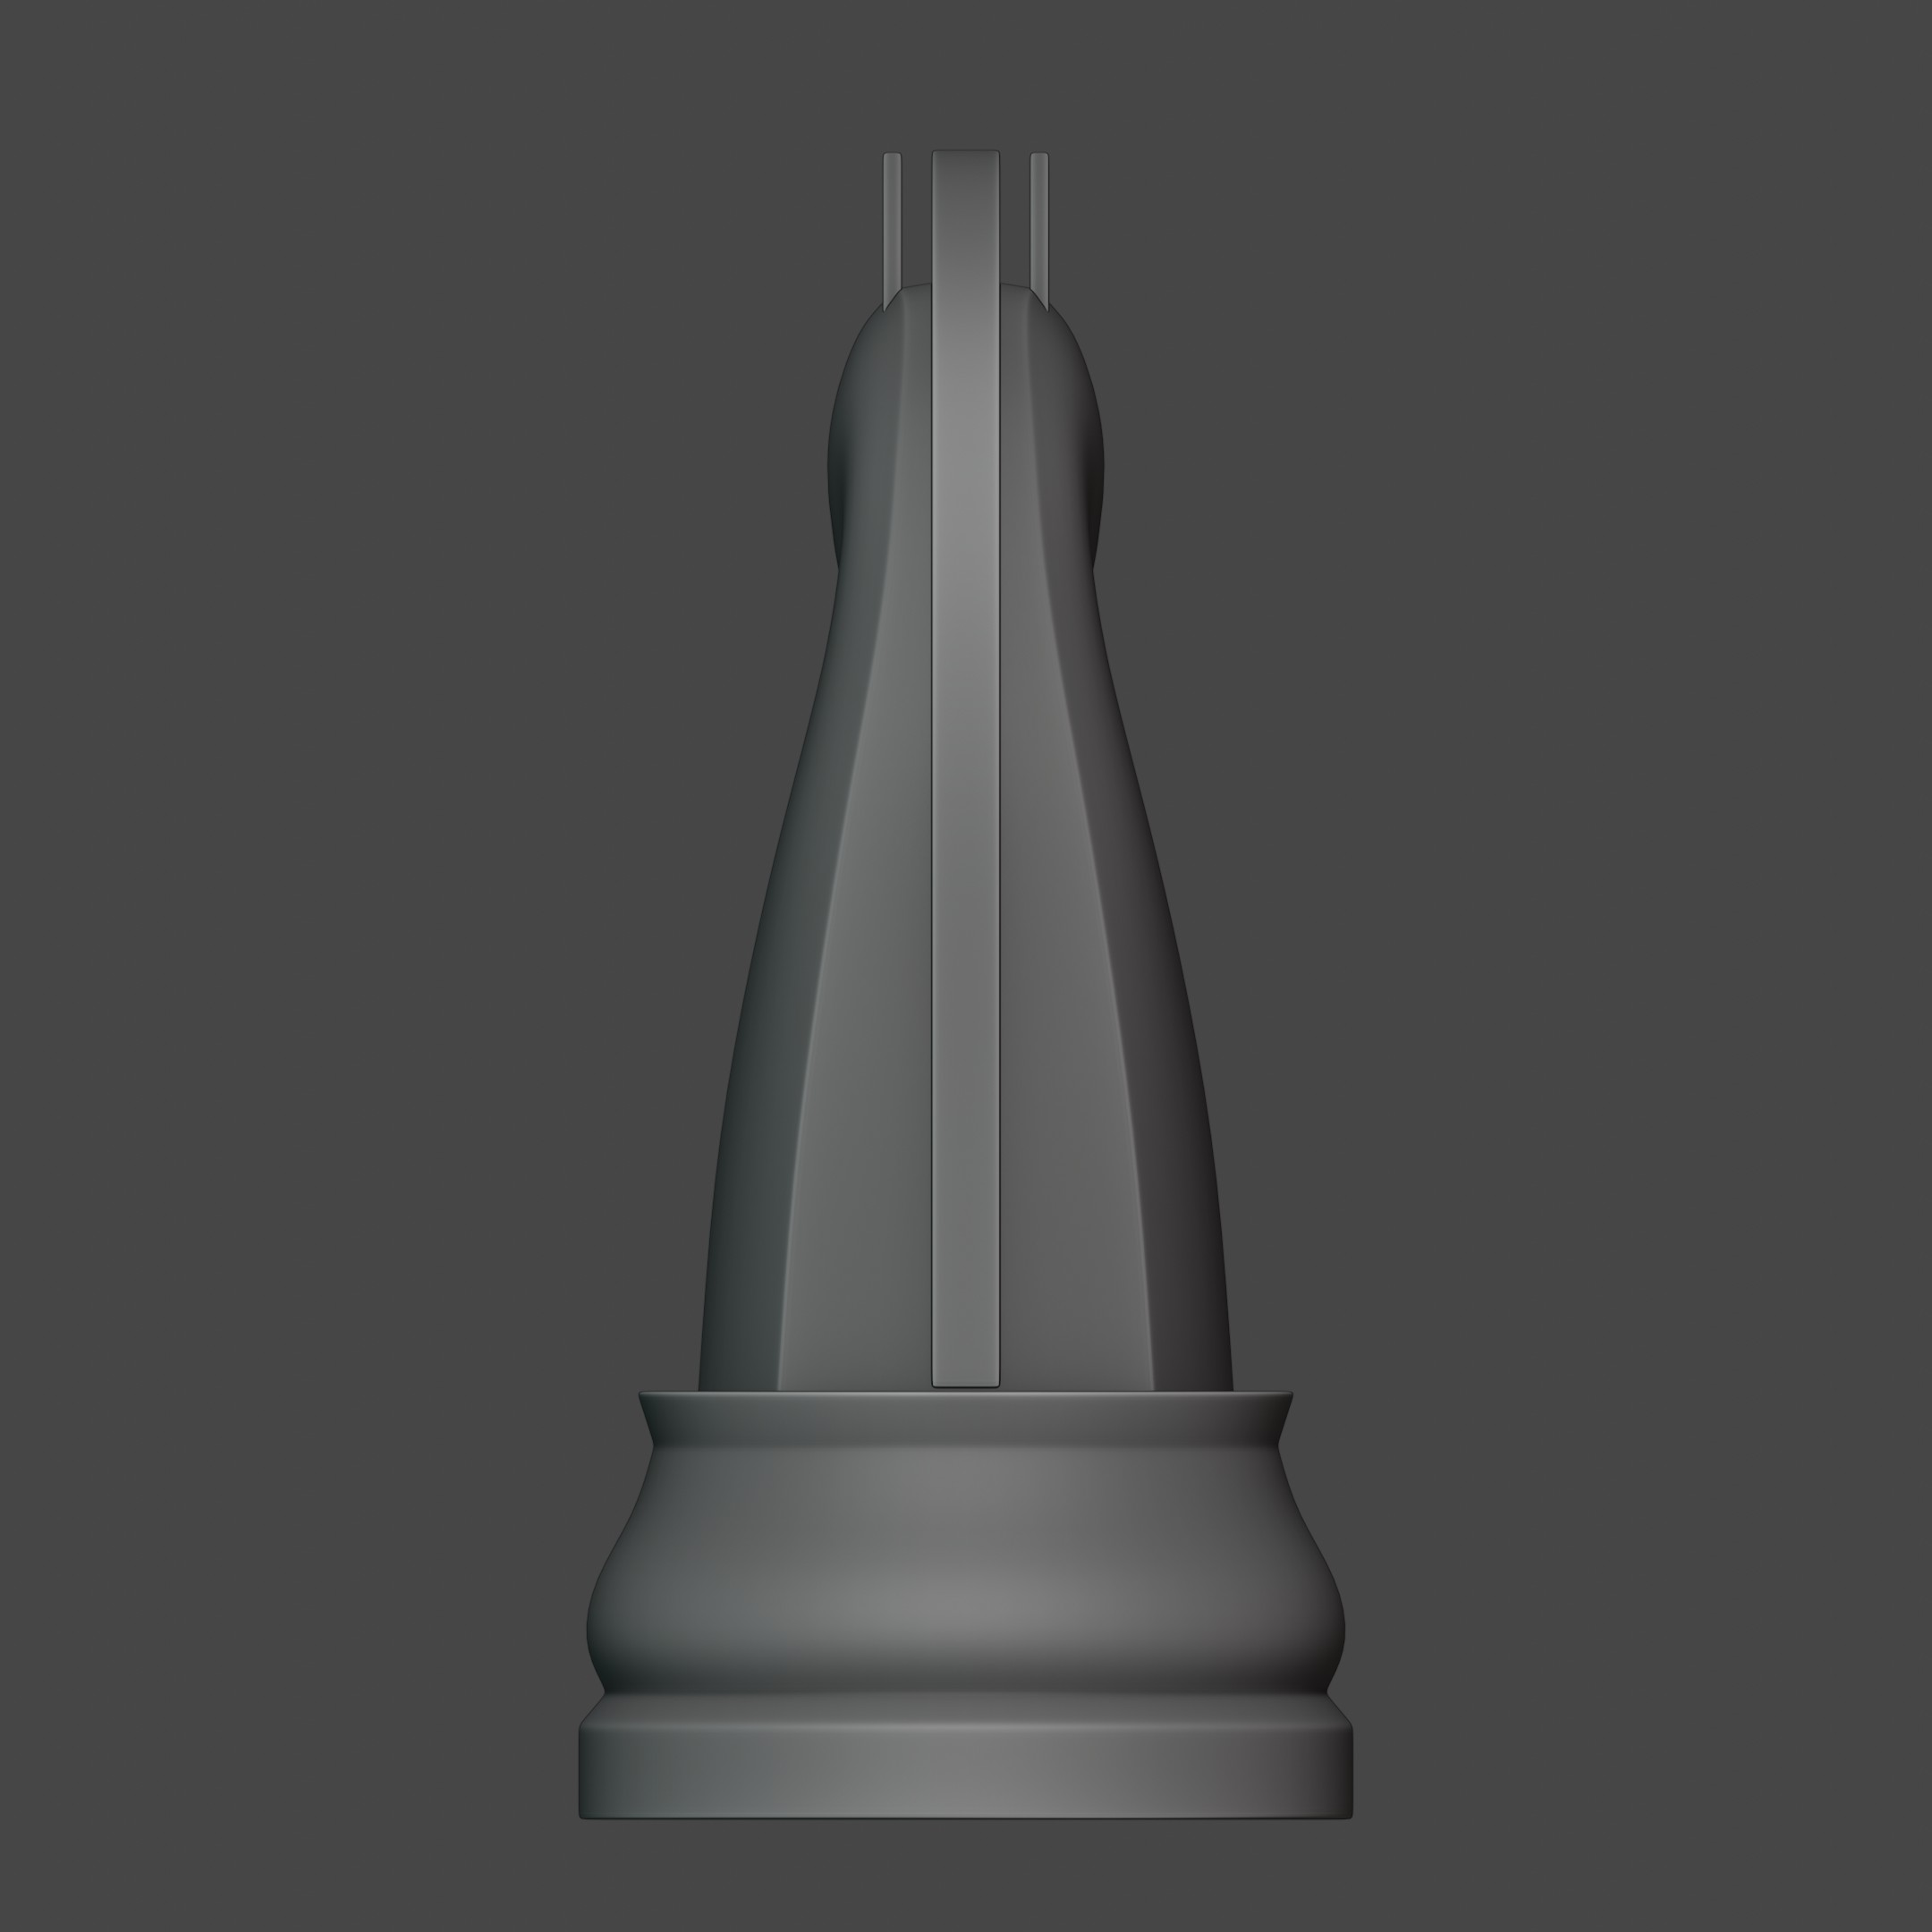
\includegraphics[width=0.3\textwidth]{ref/knight back.jpg}
\end{center}
Additionally ico-spheres where added  to piece some pieces additional detail.
\begin{center}
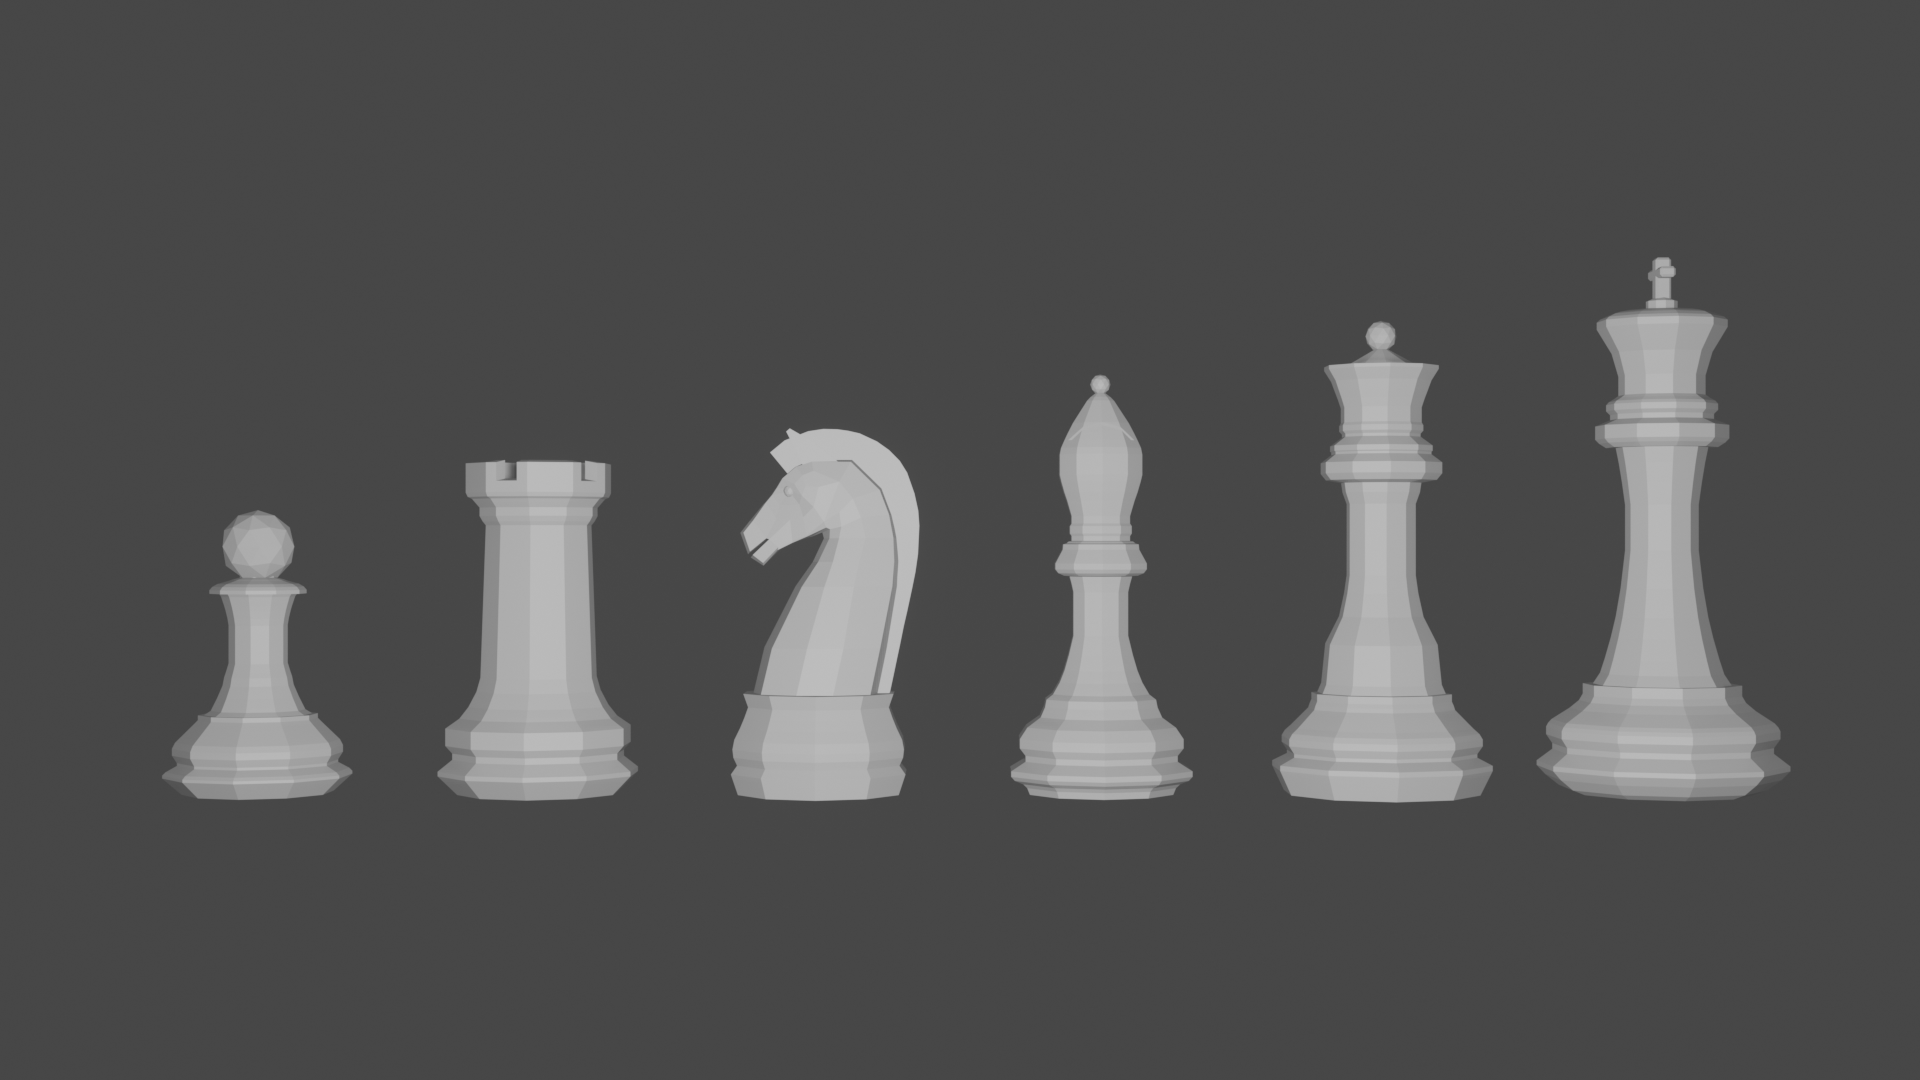
\includegraphics[width=0.5\textwidth]{Images/Pieces.png}
\end{center}
\subsubsection{Board}
\label{sec:org9e93267}
\begin{enumerate}
\item Chess board
\label{sec:orgc64f8a2}
\item Marble exterior
\label{sec:orgb95e97c}
\end{enumerate}
\subsubsection{Textures and shading}
\label{sec:orgf2a96e7}
\subsubsection{Particle effects}
\label{sec:orgcc3f50b}
\begin{enumerate}
\item Explosions
\label{sec:org2f5b2bd}
\item Confetti
\label{sec:orgf9dbb54}
\end{enumerate}
\subsubsection{Lighting}
\label{sec:org4ca82ba}
\begin{enumerate}
\item Direct
\label{sec:org7e7b9d0}
\item Indirect
\label{sec:org1989bbf}
\item Disco ball
\label{sec:org0755980}
\end{enumerate}
\subsubsection{Render engine}
\label{sec:org9398bca}
\begin{enumerate}
\item Eevee
\label{sec:org7575c9e}
\item Cycles
\label{sec:orgaa573e4}
\begin{enumerate}
\item Thank you to Jack
\label{sec:org9e6ef0f}
\end{enumerate}
\item Luxcore
\label{sec:orga6d0213}
\end{enumerate}
\subsection{Python side}
\label{sec:org20f1376}
\subsubsection{Processing games}
\label{sec:org07b117c}
\subsubsection{Unique pairing problem}
\label{sec:org6a206e2}
\subsubsection{The solution}
\label{sec:org05ca28a}
\subsubsection{Array index to world space}
\label{sec:org5ea3396}
\setchessboard{color=black,clearboard,showmover=false}
\chessboard[
pgfstyle=
{[base,at={\pgfpoint{0pt}{-0.3ex}}]text},
text= \fontsize{1.2ex}{1.2ex}\bfseries
\sffamily\getfieldnumber\currentwq,
markboard]
\begin{enumerate}
\item Abuse of this functionality
\label{sec:orgf5fd2a9}
\end{enumerate}
\subsubsection{Special moves}
\label{sec:org5bfcaa3}
\begin{enumerate}
\item Promotion
\label{sec:org9319925}
\item En passant
\label{sec:org9945573}
\item Castling
\label{sec:orgdc5ab0c}
\end{enumerate}
\subsubsection{Animation}
\label{sec:orgdbb2220}
\begin{enumerate}
\item Key frames
\label{sec:org10415ee}
\begin{enumerate}
\item Timing
\label{sec:org804b7d2}
\end{enumerate}
\item Interpolation
\label{sec:org6a70068}
\end{enumerate}
\subsection{Reproducibility}
\label{sec:org4127249}
This project was created used
\begin{itemize}
\item Blender \texttt{2.92}
\url{https://www.blender.org/}
\item Python \texttt{3.9.5} \footnote{Blender comes bundled with this version. If the system python is used
instead ensure it is above \texttt{3.7} for the \texttt{\_\_future\_\_} module.}
\url{https://www.python.org/}
\item python-chess \texttt{1.5.0} \footnote{This project requires the \texttt{Outcome} class released in \texttt{1.5.0}}
\url{https://github.com/niklasf/python-chess}
\end{itemize}
\subsubsection{Python environment}
\label{sec:org092b555}
Blender is distributed with its own python installation for consistency,
however this means that installed python modules are not present
\cite{blender-python-env}. To mitigate this the \texttt{-{}-target} flag for \texttt{pip install}
can be used to install directly to the blender python environment
\cite{pip-install-man}.
\begin{Code}
\begin{Verbatim}[]
\color[HTML]{383a42}pip install -t \char126{}/.config/blender/2.92/scripts/modules chess
\end{Verbatim}
\end{Code}

\section{Results}
\label{sec:org651a5cd}
\section{Evaluation}
\label{sec:orgaa4e938}

\newpage
\section{Appendix}
\label{sec:orgd0a78ad}
\newpage
\printbibliography
\end{document}
